%! Author = ahmed_hassanien
%! Date = 4/1/20

% Preamble
\documentclass[
    handout, % Comment to release the presentation
    aspectratio=169
]{beamer}
% Packages
\usepackage[sectionpage=progressbar,progressbar=foot]{theme/beamerthememetropolis}
\usepackage{tikz}
\usepackage{caption}
\usepackage{fontawesome}
\usepackage{hyperref}
\usepackage{listings}

% Libraries
\usetikzlibrary{positioning, shapes, backgrounds, fit}

% Global Settings
\setbeamersize{text margin left=3mm,text margin right=3.6cm}
\tikzset{
    invisible/.style = {opacity=0},
    visible on/.style = {alt={#1{}{invisible}}},
    alt/.code args = {<#1>#2#3}{\alt<#1>{\pgfkeysalso{#2}}{\pgfkeysalso{#3}}} % \pgfkeysalso doesn't change the path.
}
\captionsetup{justification = raggedright, singlelinecheck = false}

% Details
\title[Dockerization]{Dockerization}
\subtitle{\textit{Toward an Agile Infrastructure}}
%------------------------------------------------------------
%This block of code defines the information to appear in the
%Title page
\title[Containerization \& Virtualization] %optional
{Containerization \& Virtualization}

\subtitle{\textit{Toward Faster, Easier, and Automated SDLC}}

\author[Ahmed Hassanin] {
	Ahmed Hassanin \newline Lead Software Engineer \newline 
	\faGithub \space \href{https://github.com/gabrianoo}{Gabrianoo}	
	\faLinkedin \space \href{https://www.linkedin.com/in/ahmedgaber}{Ahmed Hassanien}
	\faYoutubePlay \space \href{https://youtube.com/c/GarageEducation}{Garage Education}\newline	\faEnvelope \space \href{mailto: eng.ahmedgaber@gmail.com}{eng.ahmedgaber@gmail.com} 
}


\date{\today}



%\logo{\includegraphics[height=1.5cm]{lion-logo.png}}

%End of title page configuration block
%------------------------------------------------------------

%%%%%%%%%%%%%%%%%%%%%%%%%%%%%%%%%%%%%%%%%%%%%%%%%%%%%%%%%%%%%%%%%%%%%%%%%%%
%%% Local Variables:
%%% mode: latex
%%% TeX-master: "./main"
%%% TeX-engine: xetex
%%% End:


% Document
\begin{document}

    \maketitle

    \begin{frame}{Table of contents}
        \setbeamertemplate{section in toc}[sections numbered]
        \tableofcontents[hideallsubsections]
    \end{frame}

    \definecolor{listinggray}{gray}{0.9}
\definecolor{lbcolor}{rgb}{0.9,0.9,0.9}
\lstset{
    backgroundcolor=\color{lbcolor},
    tabsize=4,
    rulecolor=,
    language=matlab,
    basicstyle=\fontsize{7}{7}\ttfamily,
    upquote=true,
    aboveskip={1.5\baselineskip},
    columns=fixed,
    showstringspaces=false,
    extendedchars=true,
    breaklines=true,
    prebreak = \raisebox{0ex}[0ex][0ex]{\ensuremath{\hookleftarrow}},
    frame=single,
    showtabs=false,
    showspaces=false,
    showstringspaces=false,
    identifierstyle=\ttfamily,
    keywordstyle=\color[rgb]{0,0,1},
    commentstyle=\color[rgb]{0.133,0.545,0.133},
    stringstyle=\color[rgb]{0.627,0.126,0.941},
}

    %----------------------------------------------------------------------------------------------------------------------%

\section{Introduction - Docker Overview}\label{sec:introduction-docker-overview}
%----------------------------------------------------------------------------------------------------------------------%

\subsection{What is docker?}\label{subsec:what-is-docker}
\begin{frame}{What is docker?}
    \begin{itemize}[<+- | alert@+>]
        \item Docker is an OS-level virtualization tool.
        \item Docker is an open platform for developing, shipping, and running applications.
        \item Docker provides tools, and a platform to manage the lifecycle of your containers:
        \begin{itemize}
            \item Develop your application and its supporting components using containers.
            \item The container becomes the unit for distributing and testing your application.
            \item When you are ready, deploy your application into your production environment, as a container or an orchestrated service.
            \item This works the same whether your production environment is a local data center, a cloud provider, or a hybrid of the two.
        \end{itemize}
    \end{itemize}
\end{frame}

\subsection{Docker Architecture}\label{subsec:docker-architecture}
\begin{frame}{Docker Architecture}
    \begin{itemize}
        \item Docker uses a client-server architecture.
        \linebreak
        \pause
        \begin{figure}[!t]
            \raggedright
            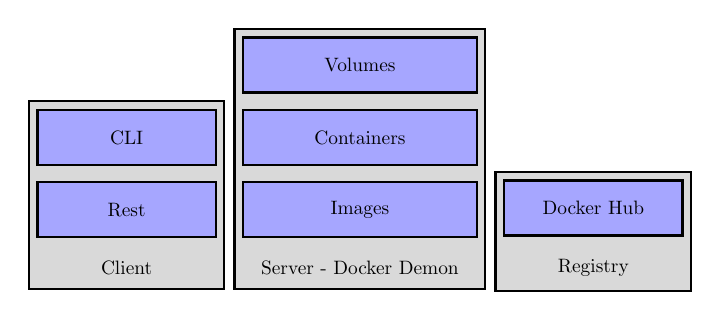
\begin{tikzpicture}[
    node/.style = {
        scale=0.70,
        node distance = 2mm,
        rectangle,
        draw = black,
        thick,
        text centered,
        minimum height = 10mm,
        minimum width = 10mm
    },
    txt/.style = {
        scale=0.70,
        node distance = 2mm,
        rectangle,
        text centered,
        minimum height = 2mm,
        minimum width = 10mm
    }
]
    \tikzstyle{layer} = [inner sep=1mm, draw=black, thick, fill= gray!30]
    \tikzstyle{vm} = [fill = gray!30]
    \tikzstyle{hw} = [fill = blue!35]
    \tikzstyle{sw} = [fill = blue!15]
    \tikzstyle{hv} = [fill = blue!5 ]
    \tikzstyle{ar} = [fill = black  ]

    %%%%%%%%%%%%%%%%%
    % Docker Client %
    %%%%%%%%%%%%%%%%%
    \node [txt, text width=3cm, visible on=<1->] (CLIENT) {Client};
    \node [node, hw, above = of CLIENT, text width=3cm, visible on=<3->] (REST) {Rest};
    \node [node, hw, above = of REST, text width=3cm, visible on=<4->] (CLI) {CLI};
    \begin{scope}[on background layer]
        \node [fit = (CLIENT) (REST) (CLI), layer, visible on=<1->] {};
    \end{scope}

    %%%%%%%%%%%%%%%%%
    % Docker Server %
    %%%%%%%%%%%%%%%%%
    \node [txt, right = of CLIENT, text width=4cm, xshift = 2mm, visible on=<5->] (SER) {Server - Docker Demon};
    \node [node, hw, above = of SER, text width=4cm, visible on=<6->] (IMG) {Images};
    \node [node, hw, above = of IMG, text width=4cm, visible on=<7->] (CON) {Containers};
    \node [node, hw, above = of CON, text width=4cm, visible on=<8->] (VOL) {Volumes};
    \begin{scope}[on background layer]
        \node [fit = (SER) (CON) (IMG) (VOL), layer, visible on=<5->] {};
    \end{scope}

    %%%%%%%%%%%%%%%%%%%
    % Docker Rigestry %
    %%%%%%%%%%%%%%%%%%%
    \node [txt, right = of SER, text width=3cm, xshift = 2mm, visible on=<9->] (REG) {Registry};
    \node [node, hw, above = of REG, text width=3cm, visible on=<10->] (HUB) {Docker Hub};
    \begin{scope}[on background layer]
        \node [fit = (REG) (HUB), layer, visible on=<9->] {};
    \end{scope}
\end{tikzpicture}
            \caption{Docker Architecture}
        \end{figure}
    \end{itemize}
\end{frame}
\begin{frame}{Docker Demon (Server)}
    \begin{itemize}[<+- | alert@+>]
        \item The Docker daemon \texttt{(dockerd)} listens for Docker API requests and manages Docker objects.
        \item A daemon can also communicate with other daemons to manage Docker services.

    \end{itemize}
\end{frame}
\begin{frame}{Docker Objects}
    \begin{itemize}[<+- | alert@+>]
        \item \textbf{Images} are a read-only template with instructions for creating a Docker container.
        \item \textbf{Containers} are a runnable instance of an image.
        \item \textbf{Volumes} are the preferred mechanism for persisting data generated by and used by Docker containers.
    \end{itemize}
\end{frame}
\begin{frame}{Docker Client}
    \begin{itemize}[<+- | alert@+>]
        \item The Docker client \texttt{(docker)} is the primary way that many Docker users interact with Docker.
        \item When you use commands such as \texttt{(docker run)}, the client sends these commands to \texttt{(dockerd)}, which carries them out.
        \item The docker command uses the Docker API and can communicate with one or more docker daemons.
    \end{itemize}
\end{frame}
\begin{frame}{Docker Registry}
    \begin{itemize}[<+- | alert@+>]
        \item A Docker registry stores Docker images.
        \item Docker Hub is a public registry that anyone can use, and by default Docker configurations looks for the images on Docker Hub.
        \item Docker Hub is not the only registry in the market, and you can use your own docker registry.
    \end{itemize}
\end{frame}
%----------------------------------------------------------------------------------------------------------------------%
    %----------------------------------------------------------------------------------------------------------------------%


\section{Docker - Short-lived containers}\label{sec:docker-short-lived-containers}
%----------------------------------------------------------------------------------------------------------------------%

\subsection{docker version}\label{subsec:docker-version}
\begin{frame}{docker version}
    \begin{itemize}
        \item \texttt{version} Show the Docker version information
        \pause
        \lstinputlisting[language=bash, linerange={3-4}]{docker/shell-samples.sh}
    \end{itemize}
\end{frame}

\subsection{docker run}\label{subsec:docker-run}
\begin{frame}{docker run}
    \begin{itemize}
        \item \texttt{run} Run a command in a new container
        \pause
        \lstinputlisting[language=bash, linerange={6-14}]{docker/shell-samples.sh}
    \end{itemize}
\end{frame}

\subsection{docker pull}\label{subsec:docker-pull}
\begin{frame}{docker pull}
    \begin{itemize}
        \item \texttt{run} Pull an image or a repository from a registry
        \pause
        \lstinputlisting[language=bash, linerange={16-30}]{docker/shell-samples.sh}
    \end{itemize}
\end{frame}

\subsection{docker ps}\label{subsec:docker-ps}
\begin{frame}{docker ps}
    \begin{itemize}
        \item \texttt{ps} List containers
        \pause
        \lstinputlisting[language=bash, linerange={47-51,79-84}]{docker/shell-samples.sh}
    \end{itemize}
\end{frame}

\subsection{docker start}\label{subsec:docker-start}
\begin{frame}{docker start}
    \begin{itemize}
        \item \texttt{start} Start one or more stopped containers
        \pause
        \lstinputlisting[language=bash, linerange={63-77}]{docker/shell-samples.sh}
    \end{itemize}
\end{frame}

\subsection{docker rm}\label{subsec:docker-rm}
\begin{frame}{docker rm}
    \begin{itemize}
        \item \texttt{rm} Remove one or more containers
        \pause
        \lstinputlisting[language=bash, linerange={85-94,109-110}]{docker/shell-samples.sh}
    \end{itemize}
\end{frame}

\subsection{docker rename}\label{subsec:docker-rename}
\begin{frame}{docker rename}
    \begin{itemize}
        \item \texttt{rename} Rename a container
        \pause
        \lstinputlisting[language=bash, linerange={112,127-134}]{docker/shell-samples.sh}
    \end{itemize}
\end{frame}

\subsection{docker images}\label{subsec:docker-images}
\begin{frame}{docker images}
    \begin{itemize}
        \item \texttt{images} List images
        \pause
        \lstinputlisting[language=bash, linerange={153-156}]{docker/shell-samples.sh}
    \end{itemize}
\end{frame}

\subsection{docker rmi}\label{subsec:docker-rmi}
\begin{frame}{docker rmi}
    \begin{itemize}
        \item \texttt{rmi} Remove one or more images
        \pause
        \lstinputlisting[language=bash, linerange={158-166}]{docker/shell-samples.sh}
    \end{itemize}
\end{frame}

\subsection{docker search}\label{subsec:docker-search}
\begin{frame}{docker search}
    \begin{itemize}
        \item \texttt{search} Search the Docker Hub for images
        \pause
        \lstinputlisting[language=bash, linerange={181-190}]{docker/shell-samples.sh}
    \end{itemize}
\end{frame}

\subsection{docker login}\label{subsec:docker-login}
\begin{frame}{docker login}
    \begin{itemize}
        \item \texttt{login} Log in to a Docker registry
        \pause
        \lstinputlisting[language=bash, linerange={192-196}]{docker/shell-samples.sh}
    \end{itemize}
\end{frame}

\subsection{docker logout}\label{subsec:docker-logout}
\begin{frame}{docker logout}
    \begin{itemize}
        \item \texttt{logout} Log out from a Docker registry
        \pause
        \lstinputlisting[language=bash, linerange={198-199}]{docker/shell-samples.sh}
    \end{itemize}
\end{frame}

\subsection{index.docker.io}\label{subsec:index.docker.io}
\begin{frame}{index.docker.io}
    \begin{itemize}
        \item \texttt{index.docker.io} is hosted on AWS :-)
        \pause
        \lstinputlisting[language=bash, linerange={201-213}]{docker/shell-samples.sh}
    \end{itemize}
\end{frame}
%----------------------------------------------------------------------------------------------------------------------%
    %----------------------------------------------------------------------------------------------------------------------%

\section{Docker - Long-lived containers}\label{sec:docker-long-lived-containers}
%----------------------------------------------------------------------------------------------------------------------%
\definecolor{listinggray}{gray}{0.9}
\definecolor{lbcolor}{rgb}{0.9,0.9,0.9}
\lstset{
    backgroundcolor=\color{lbcolor},
    tabsize=4,
    rulecolor=,
    language=matlab,
    basicstyle=\fontsize{7}{7}\ttfamily,
    upquote=true,
    aboveskip={1.5\baselineskip},
    columns=fixed,
    showstringspaces=false,
    extendedchars=true,
    breaklines=true,
    prebreak = \raisebox{0ex}[0ex][0ex]{\ensuremath{\hookleftarrow}},
    frame=single,
    showtabs=false,
    showspaces=false,
    showstringspaces=false,
    identifierstyle=\ttfamily,
    keywordstyle=\color[rgb]{0,0,1},
    commentstyle=\color[rgb]{0.133,0.545,0.133},
    stringstyle=\color[rgb]{0.627,0.126,0.941},
}

\subsection{docker detached}\label{subsec:docker-detached}
\begin{frame}{docker detached}
    \begin{itemize}
        \item \texttt{-d, --detach} Run container in background and print container ID.
        \lstinputlisting[language=bash, linerange={215-220}]{docker/shell-samples.sh}
    \end{itemize}
\end{frame}

\subsection{docker expose container port}\label{subsec:docker-expose-container-port}
\begin{frame}{docker expose container port}
    \begin{itemize}
        \item \texttt{port} List port mappings or a specific mapping for the container.
        \item \texttt{-p, --publish list} Publish a container's port(s) to the host.
        \lstinputlisting[language=bash, linerange={222-229}]{docker/shell-samples.sh}
    \end{itemize}
\end{frame}
\begin{frame}{docker bridge networking}
    \begin{figure}[!t]
        \raggedright
        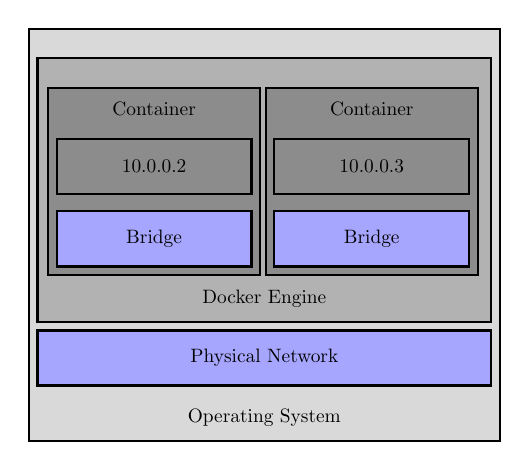
\begin{tikzpicture}[
    node/.style = {
        scale=0.70,
        node distance = 2mm,
        rectangle,
        draw = black,
        thick,
        text centered,
        minimum height = 10mm,
        minimum width = 10mm
    },
    txt/.style = {
        scale=0.70,
        node distance = 2mm,
        rectangle,
        text centered,
        minimum height = 2mm,
        minimum width = 10mm
    }
]
    \tikzstyle{layer} = [inner sep=1mm, draw=black, thick, fill= gray!30]
    \tikzstyle{de} = [inner sep=1mm, draw=black, thick, fill= gray!60]
    \tikzstyle{cr} = [inner sep=1mm, draw=black, thick, fill= gray!90]
    \tikzstyle{vm} = [fill = gray!30]
    \tikzstyle{hw} = [fill = blue!35]
    \tikzstyle{sw} = [fill = blue!15]
    \tikzstyle{hv} = [fill = blue!5 ]
    \tikzstyle{ar} = [fill = black  ]

    \node [txt, text width=8cm, visible on=<1->] (OS) {Operating System};
    \node [node, hw, above = of OS, text width=8cm, visible on=<1->] (PN) {Physical Network};
    \node [txt, above = of PN, text width=7.7cm, visible on=<1->] (DE) {Docker Engine};
    % Container 1 structure
    \node [node, hw, above = of DE, xshift = -2.0cm, text width=3.3cm, visible on=<1->] (P1) {Bridge};
    \node [node, fill= gray!90, above = of P1, text width=3.3cm, visible on=<1->] (I1) {10.0.0.2};
    \node [txt, above = of I1, text width=3.3cm, visible on=<1->] (C1) {Container};
    % Container 2 structure
    \node [node, hw, right = of P1, xshift = 1mm, text width=3.3cm, visible on=<1->] (P2) {Bridge};
    \node [node, fill= gray!90, above = of P2, text width=3.3cm, visible on=<1->] (I2) {10.0.0.3};
    \node [txt, above = of I2, text width=3.3cm, visible on=<1->] (C2) {Container};
    % Empty space
    \node [txt, above = of C1, text width=3.3cm, visible on=<1->] (T1) {};
    \node [txt, above = of T1, text width=3.3cm, visible on=<1->] (T2) {};
    % Operating system group
    \begin{scope}[on background layer]
        \node [fit = (OS) (PN) (DE) (P1) (I1) (C1) (P2) (I2) (C2) (T1) (T2), layer, visible on=<1->] {};
    \end{scope}
    % Docker Engine group
    \begin{scope}[on background layer]
        \node [fit = (DE) (P1) (I1) (C1) (P2) (I2) (C2) (T1), de, visible on=<1->] {};
    \end{scope}
    % Container 1 group
    \begin{scope}[on background layer]
        \node [fit = (P1) (I1) (C1), cr, visible on=<1->] {};
    \end{scope}
    % Container 2 group
    \begin{scope}[on background layer]
        \node [fit = (P2) (I2) (C2), cr, visible on=<1->] {};
    \end{scope}
\end{tikzpicture}
        \caption{Docker Bridge Networking}
    \end{figure}
\end{frame}

\subsection{docker show container logs}\label{subsec:docker-show-container-logs}
\begin{frame}{docker show container logs}
    \begin{itemize}
        \item \texttt{logs} Fetch the logs of a container.
        \item \texttt{-t, --timestamps} Show timestamps.
        \item \texttt{-f, --follow} Follow log output.
        \lstinputlisting[language=bash, linerange={231-239}]{docker/shell-samples.sh}
    \end{itemize}
\end{frame}

\subsection{docker restart container}\label{subsec:docker-restart-container}
\begin{frame}{docker restart}
    \begin{itemize}
        \item \texttt{restart} Restart one or more containers.
        \item \texttt{-t, --time int} Seconds to wait for stop before killing the container (default 10).
        \lstinputlisting[language=bash, linerange={241-249}]{docker/shell-samples.sh}
    \end{itemize}
\end{frame}

\subsection{docker stop container}\label{subsec:docker-stop-container}
\begin{frame}{docker stop container}
    \begin{itemize}
        \item \texttt{stop} Stop one or more running containers.
        \item \texttt{-t, --time int} Seconds to wait for stop before killing it (default 10).
        \lstinputlisting[language=bash, linerange={250-260}]{docker/shell-samples.sh}
    \end{itemize}
\end{frame}

\subsection{docker kill container}\label{subsec:docker-kill-container}
\begin{frame}{docker kill container}
    \begin{itemize}
        \item \texttt{Kill} Kill one or more running containers.
        \lstinputlisting[language=bash, linerange={262-265}]{docker/shell-samples.sh}
    \end{itemize}
\end{frame}

\subsection{docker stats}\label{subsec:docker-stats}
\begin{frame}{docker stats}
    \begin{itemize}
        \item \texttt{stats} Display a live stream of container(s) resource usage statistics.
        \item \texttt{-a, --all} Show all containers (default shows just running).
        \item \texttt{--no-stream} Disable streaming stats and only pull the first result.
        \lstinputlisting[language=bash, linerange={267-274}]{docker/shell-samples.sh}
    \end{itemize}
\end{frame}

\subsection{docker top}\label{subsec:docker-top}
\begin{frame}{docker top}
    \begin{itemize}
        \item \texttt{top} Display the running processes of a container.
        \lstinputlisting[language=bash, linerange={276-281}]{docker/shell-samples.sh}
    \end{itemize}
\end{frame}

\subsection{docker pause and unpause}\label{subsec:docker-pause-and-unpause}
\begin{frame}{docker pause and unpause}
    \begin{itemize}
        \item \texttt{pause} Pause all processes within one or more containers.
        \item \texttt{unpause} Unpause all processes within one or more containers.
        \lstinputlisting[language=bash, linerange={283-294}]{docker/shell-samples.sh}
    \end{itemize}
\end{frame}

\subsection{docker exec}\label{subsec:docker-exec}
\begin{frame}{docker exec}
    \begin{itemize}
        \item \texttt{exec} Run a command in a running container.
        \item \texttt{-i, --interactive} Keep STDIN open even if not attached.
        \item \texttt{-t, --tty} Allocate a pseudo-TTY.
        \lstinputlisting[language=bash, linerange={296-300,302-305,307-309}]{docker/shell-samples.sh}
    \end{itemize}
\end{frame}

\subsection{docker cp}\label{subsec:docker-cp}
\begin{frame}{docker cp}
    \begin{itemize}
        \item \texttt{cp} Copy files/folders between a container and the local filesystem.
        \lstinputlisting[language=bash, linerange={317-319}]{docker/shell-samples.sh}
    \end{itemize}
\end{frame}

\subsection{docker wait}\label{subsec:docker-wait}
\begin{frame}{docker wait}
    \begin{itemize}
        \item \texttt{wait} Block until one or more containers stop, then print their exit codes.
        \lstinputlisting[language=bash, linerange={321-324}]{docker/shell-samples.sh}
    \end{itemize}
\end{frame}

\subsection{docker attach}\label{subsec:docker-attach}
\begin{frame}{docker attach}
    \begin{itemize}
        \item \texttt{attach} Attach local standard input, output, and error streams to a running container.
        \lstinputlisting[language=bash, linerange={326}]{docker/shell-samples.sh}
    \end{itemize}
\end{frame}
%----------------------------------------------------------------------------------------------------------------------%
    %----------------------------------------------------------------------------------------------------------------------%


\section{Docker - More than one container app}\label{sec:more-than-one-container-app}
%----------------------------------------------------------------------------------------------------------------------%

\subsection{Docker default bridge}\label{subsec:docker-default-bridge}
\begin{frame}{Docker default bridge}
    \begin{itemize}
        \item What if we have an application with more than one container.
        \item Ex; WordPress rich content management system uses apache httpd and mysql servers.
        \item \texttt{-e, --env list} Set environment variables.
        \lstinputlisting[language=bash, linerange={329-334}]{docker/shell-samples.sh}
    \end{itemize}
\end{frame}

\subsection{User-defined bridge}\label{subsec:user-defined-bridge}
\begin{frame}{User-defined bridge}
    IMAGE GOES HERE
\end{frame}
\begin{frame}{User-defined bridge}
    \begin{itemize}
        \item User-defined bridges provide automatic DNS resolution between containers.
        \item User-defined bridges provide better isolation.
        \item Containers can be attached and detached from user-defined networks on the fly.
        \item Each user-defined network creates a configurable bridge.
        \item Linked containers on the default bridge network share environment variables.
    \end{itemize}
\end{frame}

\subsection{Docker Network Commands}\label{subsec:docker-network-commands}
\begin{frame}{Docker Network Commands}
    \begin{itemize}
        \item \texttt{create} Create a network.
        \item \texttt{ls} List networks.
        \item \texttt{connect} Connect a container to a network.
        \item \texttt{inspect} Display detailed information on one or more networks.
        \item \texttt{rm} Deletes one or more networks.
        \lstinputlisting[language=bash, linerange={336-344}]{docker/shell-samples.sh}
    \end{itemize}
\end{frame}
\end{document}